\documentclass[AMA,STIX1COL]{WileyNJD-v2}
\usepackage{graphicx}
\usepackage{wrapfig}
\usepackage{lscape}
\usepackage{rotating}
\usepackage{epstopdf}
\usepackage{float}

\articletype{Article Type}%

\received{26 April 2016}
\revised{6 June 2016}
\accepted{6 June 2016}

\raggedbottom

\begin{document}

\title{Bayesian hierarchical mixture cure modelling \protect\thanks{title footnote.}}

\author[1]{Nathan Green*}

\author[2,3]{Gianluca Baio}

\author[3]{Author Three}

\authormark{N Green \textsc{et al}}

\address[1]{\orgdiv{Department of Statistical Science}, \orgname{UCL}, \orgaddress{\state{London}, \country{UK}}}

\address[2]{\orgdiv{Org Division}, \orgname{Org Name}, \orgaddress{\state{State name}, \country{Country name}}}

\address[3]{\orgdiv{Org Division}, \orgname{Org Name}, \orgaddress{\state{State name}, \country{Country name}}}

\corres{*Nathan Green \email{n.green@ucl.ac.uk}}

\presentaddress{}

\abstract[Summary]{This paper is concerned with the ...}

\keywords{Bayesian, survival analysis, oncology}

\jnlcitation{\cname{%
\author{Green N.}, and
\author{G. Baio}} (\cyear{2021}), 
\ctitle{}, \cvol{2017;00:1--6}.}

\maketitle

\footnotetext{\textbf{Abbreviations:} MCM, mixture cure model}


\section{Introduction}\label{sec:intro}

{\it set the scene}\\
better diagnosis and screening has lead to more cured cancer patients.
Note that 'cured' means has a general population mortality rate.
Cure models split patients in to two (or more?) groups: cured or not.
Individual are subject to one to two source of risk.
There are several types of cure models.
(see \cite{Yu2013} for a comparison and guidance with application to oncology.)


Immuno-oncologic (IO) studies for melanoma therapies, such as {\it ipilimumab}, {\it nivolumab}, and dual {\it nivolumab} and {\it ipilimumab} combination,
have indicated that survival curves "plateau" (a considerable proportion of patients are "long-term survivors").
Cure models are a special type of survival analysis where this "cure fraction" (the underlying proportion of responders to treatment/long-term survivors) is accounted for.
Cure models estimate the cure fraction, in addition to a parametric survival function for patients that are not cured.
The mortality risk in the cured patients is informed by a background mortality rate.
The population that is not cured is subject both to background mortality and to additional mortality from their cancer, estimated using a parametric survival model.
\cite{Amico2018}

Why are MCM important, specifically in health economics?
more prevalent in HEA
plateau in events

Brief review of existing applications


BMC to give background...

limitations?
Q. can we do better?
i) PFS from OS
ii) pooled fraction

Our innovative proposal:
In this paper we ...joint model of PFS and OS, which has the double advantage of borrowing information
(eg the likely more mature PFS data to inform the highly censored OS)
*and* obtaining a pooled cure rate.

We will take a Bayesian approach; for a non-cure fraction model survival analysis in health economics \cite{Demiris2006,Jackson2010}.

A frequentist multi-level modelling approach in mixture cure modelling has been studies previously \cite{Lai2009}.
They use random effects to model multilevel clustering structure in the linear predictors in both hazard function and cured probability parts.

However, to our knowledge there has been no Bayesian fully-parametric mixture cure model with a multi-level modelling structure for event types.

Correlation between random effect in the uncured survival and cure fraction has also been investigated using a bivariate Normal distribution \cite{Lai2008}.
In our analysis, we shall assume that the uncured survival is independent of the cure fraction covariates, namely the treatment.

A suite of distributions given in NICE guidelines for health technology assessments (HTA) [ref] are
Exponential, Weibull, Gompertz, Log-logistic, Log-Normal and xxx.
This has been interpreted as meaning all of these distributions should be modelled with a given data set.
This prescriptive approach does not take into account what we know {\it a priori} about the problem.
In reality, a subset of these distributions will be more appropriate for the problem.

% software
This analysis has been carried-out using the Stan inference engine
\cite{carpenter2017stan} called from R \cite{Rcoreteam} on a Windows 10 PC.
The details of the algorithm can be found in the Appendix.
The packaged code is in a generalisable framework and can be downloaded from here.


\section{Motivating example}\label{sec:example}
Our motivating example concerns
long term
different cut points

\subsection{Checkmate 067 trial data}
The data source for the analysis is the patient-level data from the CheckMate 067 trial [ref?].
Our dataset contains $n = 945$ subjects (8 with a missing treatment indicator, i.e. the actual treatment received).
The treatment groups are as  follows:
\begin{description}
\item[Nivolumab monotherapy] 3 mg/kg intravenous (IV) once every 2 weeks (Q2W). 313 patients were treated (203 PFS events and 175 OS events).
Median PFS and OS are 6.93 months (95\% confidence interval (CI) 5.32 - 10.41) and 36.9 months (95\% CI 31.24 - 60.9), respectively. {\it should time be in months/days?}
\item[Ipilimumab monotherapy] 3 mg/kg IV once every 3 weeks (Q3W) for a total of 4 doses.
311 patients have been treated (261 PFS events and 228 OS events). Median PFS and OS are 2.86 months (95\% CI 2.79 - 3.29) and 20.0 months (95\% CI 17.22 - 25.6), respectively.
\item[Combined nivolumab with ipilimumab] 1 mg/kg IV and 3 mg/kg IV Q3W for 4 doses followed by nivolumab 3 mg/kg IV Q2W.
313 patients were treated (182 PFS events and 151 OS events). Median PFS is 11.50 months (95\% CI 9.26 - 20.80) and median OS not reached. 
\end{description}


{\it How it compares with dataset prevalent in our field/applications? BMS?}

%
\section{Methods}\label{sec:methods}

\begin{figure}
\centering
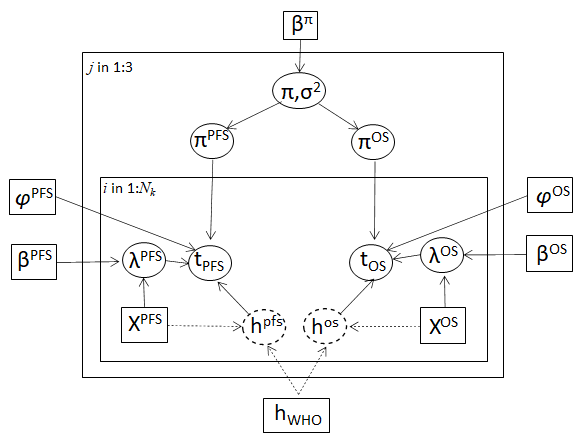
\includegraphics[width=0.6\linewidth]{DAG_with_Tx.png}
\caption{\label{fig:hier_dag} Hierarchical cure fraction DAG for PFS and OS.
Cured patients have fixed hazards.
The distribution of times for uncured patient regresses on covariates for the rate parameter and $\phi$ may be a vector of length $\geq 1$ depending on the distribution.
Censoring has been omitted for brevity.}
\end{figure}

\subsection{The standard mixture cure model} \label{section:basic_model}
The standard mixture cure model (MCM) (sometimes called a long-term survival model), which is the basis of the proposed model,
is a type of cure model where survival is modelled as a mixture of two groups of patients:
those who are cured and those who are not.
In the simplest case this consists of those who will never experience the event of interest and those who remain at risk of the event.
The more general case adopted in this paper is when cured does not mean that an individual will never experience the event of interest but the chance of doing so reverts to a general or background population probability e.g. all-cause mortality.
The combined survival for a population with a cure fraction can be written as follows

\begin{equation}
\label{eqn:mcm}
S(t, x) = S_b(t, x) [\pi(x) + (1 - \pi(x)) S_u(t, x)],
\end{equation}
\\
\noindent
where $S(t)$ denotes survival at time $t$,
$S_b(t, x)$ is a function of the background mortality at time $t$ conditional on covariates $x$,
% some papers denote \pi as _uncured_ fraction
$\pi(x)$ denotes the probability of being cured conditional on covariates $x$,
and $S_u(t, x)$ is a function of the (excess) mortality due to cancer at time $t$ conditional on covariates $x$.

All treatments are included in the same model with the following fixed effect model on the global cure fraction
$$
\text{logit}(\pi) = \beta^{\pi}_1 + \beta^{\pi}_2 TRT,
$$
where $\beta^{\pi}_1$ represents an intercept and $\beta^{\pi}_2$ is the regression coefficient for the $TRT$ covariate.
Note that we could also include a frailty term for individual $i$.
The treatment identifier is included in the covariate vector $x$.
We will assume without loss of generalisability that all individuals have all treatments.

In many mixture cure fraction analyses the survival associated with the uncured fraction of the population is represented by a Cox proportional hazard model.
This means that the baseline hazard is left unspecified but still the coefficients can be estimated.
However, we are concerned with the application of cure models to a health economics context.
In this case it is important to determine life-time survival in order to calculate total health impact measures such as quality-adjusted life-years (QALY) and life-years lost (LYL).
Therefore, the semi-parametric approach is inadequate because we must extrapolate beyond the observed data.
In this paper we will adopt a fully-parametric model for the uncured survival.

It is common to have $S_b(t, x) = 1$ which is reasonable in the short-term.
However, we are focused on the full life-course of an individual and so include this as a general population all-cause mortality.


\subsubsection{Likelihood}
There are two main approaches for formulating the MCM likelihood.
The first is to consider the group membership of an individual to either cured or uncured as missing data [ref].
Then the likelihood is defined in terms of the complete data and the augmented data are estimated along with the other parameters in the model, commonly using an EM algorithm.
The second approach is not to be concerned with the individual classification but rather estimate a single cure fraction for the whole sample.
This is the method used in this paper.

Let $T_{ij}$ be a non-negative event time and $C_{ij}$ be a censoring time for the $i$th individual and treatment $j$.
Then define the censoring indicator $\delta_{ij} = I(T_{ij} < C_{ij})$ and variable denoting the observed survival time $t_{ij} = \min(T_{ij}, C_{ij})$.
Either $\delta_{ij} = 1$ or $0$ denoting an event or censored observation at $t_{ij}$.
The observed data on the $i$th individual and treatment $j$ are thus
$\mathcal{O}_{ij} = (t_{ij}, \delta_{ij}, \boldsymbol{x}_{ij}),\; i = 1, \ldots, N, \; j = 1, \ldots, m_i \leq M$,
where $\boldsymbol{x}_{ij} = (x_{ij1}, \ldots, x_{ijS})$ is the individual covariate vector.
Covariates may be experimental (e.g. treatment assignment) or prognostic factors.

The likelihood of the standard survival is

\begin{equation*}
L(\boldsymbol{\beta} | \mathcal{O}) =
\prod_{i,j} S(t_{ij} | \boldsymbol{x}_{ij}) h(t_{ij} | \boldsymbol{x}_{ij})^{\delta_{ij}}
\end{equation*}
Log-likelihood is therefore
$$
\mathnormal{l}(\boldsymbol{\beta} | \mathcal{O}) =
\sum_{ij} \log(S(t_{ij} | \boldsymbol{x}_{ij})) + \delta_{ij} \log(h(t_{ij} | \boldsymbol{x}_{ij}))
$$
Plugging this directly into the mixture cure equation in (\ref{eqn:mcm}) gives

\begin{equation}
\label{separate_lik}
\mathnormal{l}(\boldsymbol{\beta^{\pi}}, \boldsymbol{\beta^{u}}, \boldsymbol{\beta_b} | \mathcal{O}) =
\sum_{ij} \log\left( S_b(t_{ij} | \boldsymbol{x}_{ij}) h^*(t_{ij} | \boldsymbol{x}_{ij})^{\delta_{ij}} \left[\pi(x_{ij}) +
   (1 - \pi(x_{ij})) S_u(t_{ij} | \boldsymbol{x}_{ij}) h_u(t_{ij} | \boldsymbol{x}_{ij})^{\delta_{ij}} \right] \right)
\end{equation}

% If we assume that the cured component is the Exponential survival model
% then the non-cured component can be thought of in similar terms to the
% cumulative incidence function. That is, the probability of an event is
% the combined probability of surviving both events (e.g. for OS,
% all-cause and cancer mortality) and then experiencing either i.e.
% dropping the $S$ dependencies for brevity

% \begin{equation}
% \label{eqn:surv_pdf_exp}
% S_b S_u (h^*)^{\delta} + S_b S_u (h_u)^{\delta} = S_b S_u (h^* + h_u)^{\delta}
% \end{equation}

\subsubsection{Background survival}
We used the World Health Organisation (WHO) life tables by country for the latest year available of 2016
\cite{wholifetables} to inform the background mortality $S_b(t, x)$ in (\ref{eqn:mcm}).
The baseline hazards are the expected mortality rate for each
patient at the age at which they experience the event. The mortality
data are country, age and gender adjusted, thus providing a granular account of
the different patient profiles in the trial.
The WHO reports conditional probabilities of death in 5-year intervals until age 85.
A constant annual mortality rate is reported for individuals over 85.
They assumed that no-one lives beyond 100 years.

In a Bayesian analysis there are alternative ways in which we could
model the background mortality.
For this work we shall use WHO hazard point estimates as fixed and known.
We could consider the WHO estimates to provide sufficiently accurate estimates
given the sample size and so incorporating uncertainty is not necessary.
This also forces consistency across fits.
Denote the WHO estimates for individual $i$ and treatment $j$ as
$\hat{f}_{ij}, \hat{S}_{ij}, \hat{h}_{ij}$ for the density,
survival and hazard respectively, and include these in the set of observed
data $\mathcal{O}$.

This gives the modified likelihood from (\ref{separate_lik})
\begin{equation*}
\mathnormal{l}(\boldsymbol{\beta^{\pi}}, \boldsymbol{\beta^{u}}, \boldsymbol{\beta_b} | \mathcal{O}) =
\sum_{ij} \log\left( \hat{S}_{ij} \hat{h}_{ij}^{\delta_{ij}} \left[\pi(x_{ij}) +
   (1 - \pi(x_{ij})) S_u(t_{ij} | \boldsymbol{x}_{ij}) h_u(t_{ij} | \boldsymbol{x}_{ij})^{\delta_{ij}} \right] \right)
\end{equation*}

{\it Sharples ref re Gamma process?}

% \subsubsection{Bayesian inference}
% Using the likelihood function defined above and prior distributions on
% uncertain parameters, we can specify the posterior distribution.
% Defining $g_u$ as the prior distribution for the coefficients of the
% uncured fraction $\beta^u$ and $g_*$ as the prior distribution for the
% coefficients of the cured fraction $\beta_b$, then the general form of
% the posterior distribution can be written as follows.

% \begin{equation}
% \label{eqn:basic_posterior}
% p(\boldsymbol{\beta^{\pi}}, \boldsymbol{\beta^u}, \boldsymbol{\beta_b} | \mathcal{O}) \propto
% L(\boldsymbol{\beta^{\pi}}, \boldsymbol{\beta^{u}}, \boldsymbol{\beta_b} | \mathcal{O}) f(\boldsymbol{\beta}^{\pi}) g_{u}(\boldsymbol{\beta^{u}})g_*(\boldsymbol{\beta_b})
% \end{equation}


\subsection{The hierarchical mixture cure model}
{\it PFS and OS are correlated\\
theres information in one we can use to improve the inference in the other\\
follow-up time can be relatively short and so in this case it is more important to make use of what information we have\\
in particular OS is longer than PFS so will have more censoring}\\

Extend the observed data to include multiple event types
i.e. for the $i$th individual, $j$th treatment and $k$th event type 
$\mathcal{O} = (t_{ijk}, \delta_{ijk}, \boldsymbol{x}_{ij}), \; k = 1, \ldots, K$.
In our motivating example $K = 2$ for progression-free survival and overall survival.
The set of covariates used can be different for each $k$ and $\pi$.

The likelihood for an individual is the product of the separate likelihood functions, so from (\ref{separate_lik}),
$$
L(\boldsymbol{\beta^{\pi}}, \boldsymbol{\beta^1}, \ldots, \boldsymbol{\beta^K}, \boldsymbol{\beta_b} | \mathcal{O}) =
\prod_k L(\boldsymbol{\beta^{\pi}}, \boldsymbol{\beta^{k}}, \boldsymbol{\beta_b} | \mathcal{O})
$$
A multilevel frailty cure fraction model for the latent variable formulation was considered by \cite{Tawiah2020}.
A related generalisation by \cite{Balogun2020} consider a single event type but multiple co-infections with different cure fractions,
similar to how we have different cure fractions for each treatment.

How should we represent the cure fraction when there are multiple event times?
There are two obvious ways to represent the uncertainty about the cure fraction in the model.

The first is to specify the cure fraction directly using a
$\pi \sim \text{Beta}(a_{cf}, b_{cf})$ prior, most uninformative as a uniform
$\text{Beta}(1,1)$. The parameters can be obtained via transformation of mean
and standard deviation to allow a more natural scale for elicitation.

Alternatively, we may specify the uncertainty on the real line with a
Normal distribution and then transform to the probability scale.
A further consideration is how to represent the cure fraction so to
share information between the OS and PFS data. We will investigate 3
alternatives.

\begin{description}
    \item[Pooled] Assume that the cure fraction is the same for all event types
    $$
    \text{logit}(\pi_k) \sim \text{N}(\mu_{cf}, \sigma_{cf}^2), \; k = 1, \ldots, K.
    $$
    \item[Separate] Model each independently.
    $$
    \text{logit}(\pi_k) \sim \text{N}(\mu_k, \sigma_k^2), \; k = 1, \ldots, K.
    $$
    \item[Hierarchical] Assume exchangeability between all event types
    $$
    \pi \sim \text{N}(\mu_{cf}, \sigma_{cf}^2), \;\;  
    \text{logit}(\pi_k) \sim \text{N}(\pi, \sigma_k^2), \; k = 1, \ldots, K.  
    $$
\end{description}

% \subsubsection{Posterior distribution}
% The final posterior is
% \begin{equation}
% \label{eqn:basic_posterior}
% p(\boldsymbol{\beta^{\pi}}, \boldsymbol{\beta^{1}}, \ldots, \boldsymbol{\beta^{K}}, \boldsymbol{\beta_b} | \mathcal{O}) \propto
% L(\boldsymbol{\beta^{\pi}}, \boldsymbol{\beta^{1}}, \ldots, \boldsymbol{\beta^{K}}, \boldsymbol{\beta_b} | \mathcal{O})
%     f(\boldsymbol{\beta}^{\pi}) g_*(\boldsymbol{\beta_b}) \prod_k g_{k}(\boldsymbol{\beta^{k}})
% \end{equation}

\subsubsection{Prior specification for OS, PFS model}
The choice of priors should be informed by expert opinion.
We specify vague priors on log-scale for the coefficients of the OS and PFS rates.
Centering the ages, the baseline is $\beta_0^{PFS} \sim \text{Normal}(0, 100),\; \beta_0^{OS} \sim \text{Normal}(0, 100)$
and for age $\beta_{age}^{PFS} \sim \text{Normal}(0, 100),\; \beta_{age}^{OS} \sim \text{Normal}(0, 100)$.
This corresponds to median survival time of xxx.
We don't wish to apply covariate effect to the other parameters of the OS and PFS time distributions so we specify the priors directly on the parameter
e.g for the Weibull distribution shape parameter $\nu \sim \text{Gamma}(2, 2)$. 
The level-one cure fraction is modelled as a fixed effect linear regression with logistic link and coefficient priors $\alpha \sim \text{Normal}(0, 100)$.
The level-two cure fraction distribution for OS and PFS have logistic-normal priors for the probabilities with variances
$\sigma^2_{PFS} \sim \text{Gamma}(2, 2),\; \sigma^2_{OS} \sim \text{Gamma}(2, 2)$.


The background is taken directly from the WHO life-tables.
However, it is believed that the patients in the trial have a worse background survival than the average individual in the general population.
Using only the complete responders in the sample, who are clinically confirmed as cured, it is possible to obtain a posterior distribution for a hazard ratio between these and a WHO estimate baseline.
This can serve as a prior in the main model in a two-step approach.
Alternatively, prior belief could be defined explicitly using expert knowledge.
This could be elicited directly for the hazard ratio or on a natural scale, such as mean life time, and transformed.

{\it should the complete responders even be included in the main model? we know that they aren't uncured. If they enter via the background adjustment why double-count them?}


\subsubsection{Performance measures}
WAIC, LOO\\
$\Delta S$ at months $t = 10, 20, 30, ...$\\
clinical significant vs statistical significant differences.
hazard ratio?\\
median/mean survival?



\section{Application}\label{sec:application}

{\it Back to BMS data and results, with various scenarios/distributions and all the plots and tables, similar to the ones already provided.}

\begin{sidewaysfigure}[H]
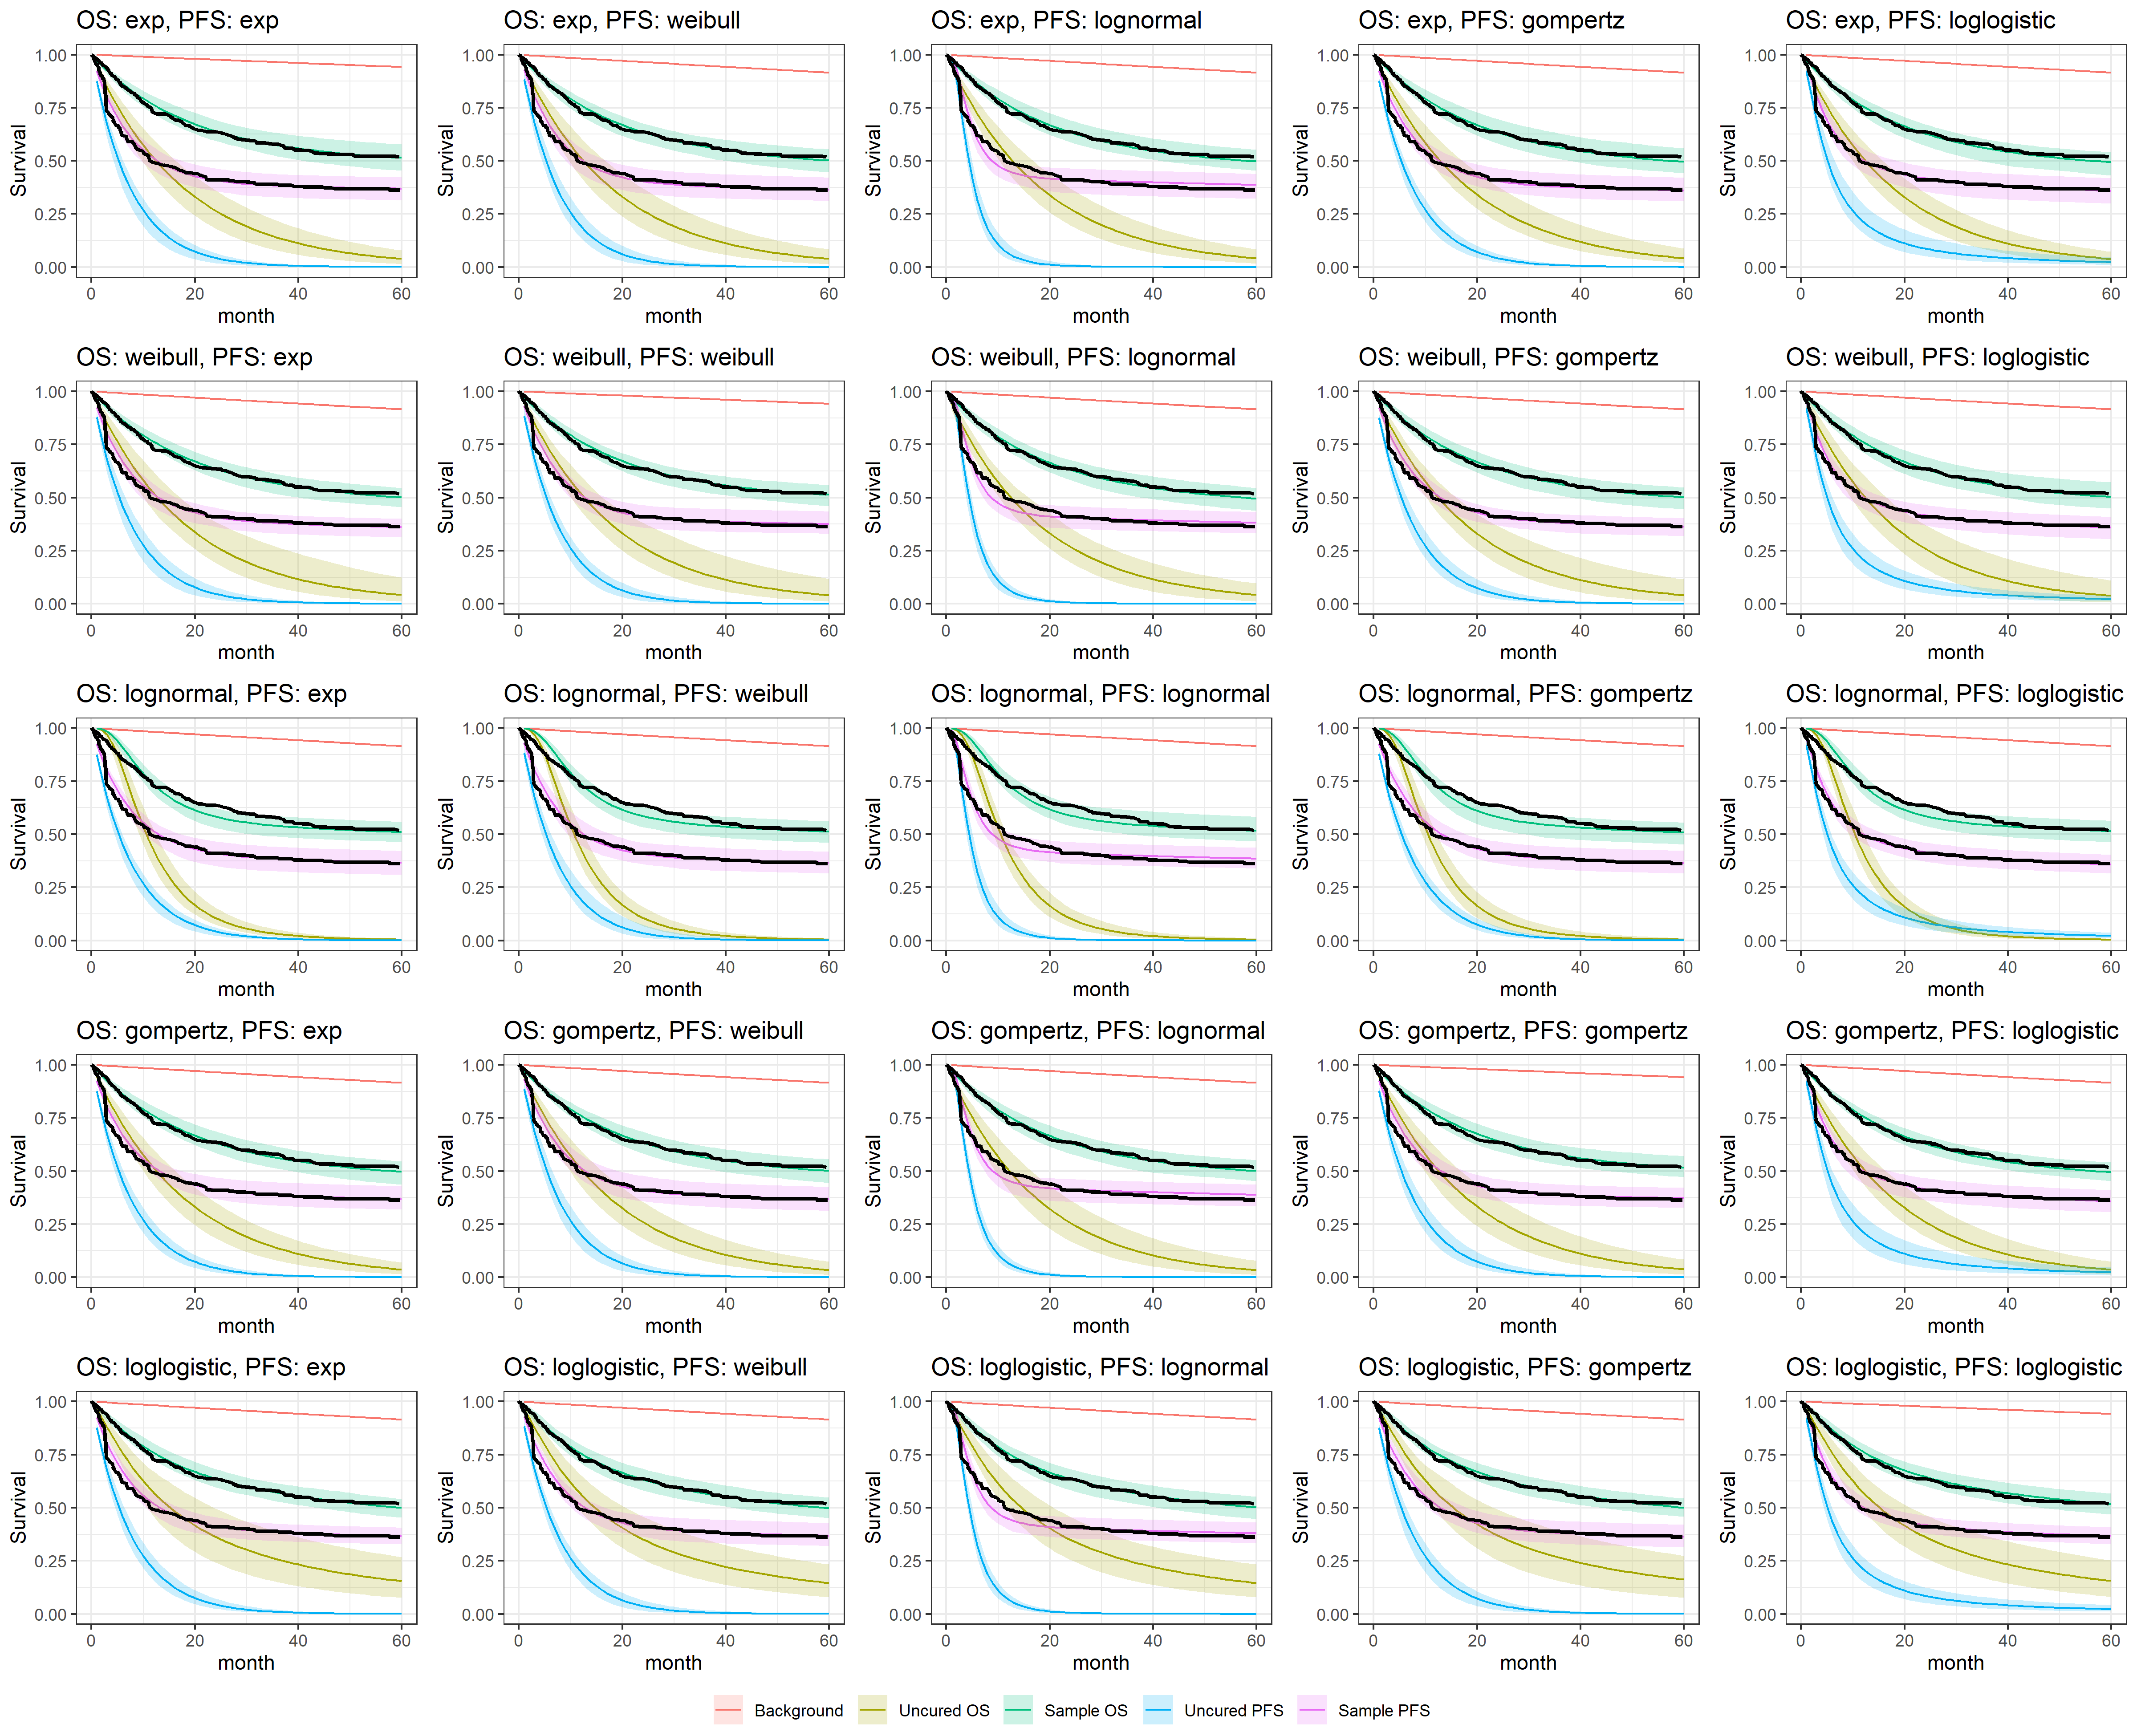
\includegraphics[width=0.9\linewidth]{plot_S_grid.png}
\caption{\label{fig:S_grid_ipi_nivo} Posterior survival curves for exponential, weibull, gompertz, log-logistic and log-Normal uncured fraction for OS and PFS events and {\it nivolumab} and {\it ipilimumab} combination treatment.}
\end{sidewaysfigure}

\begin{sidewaysfigure}[H]
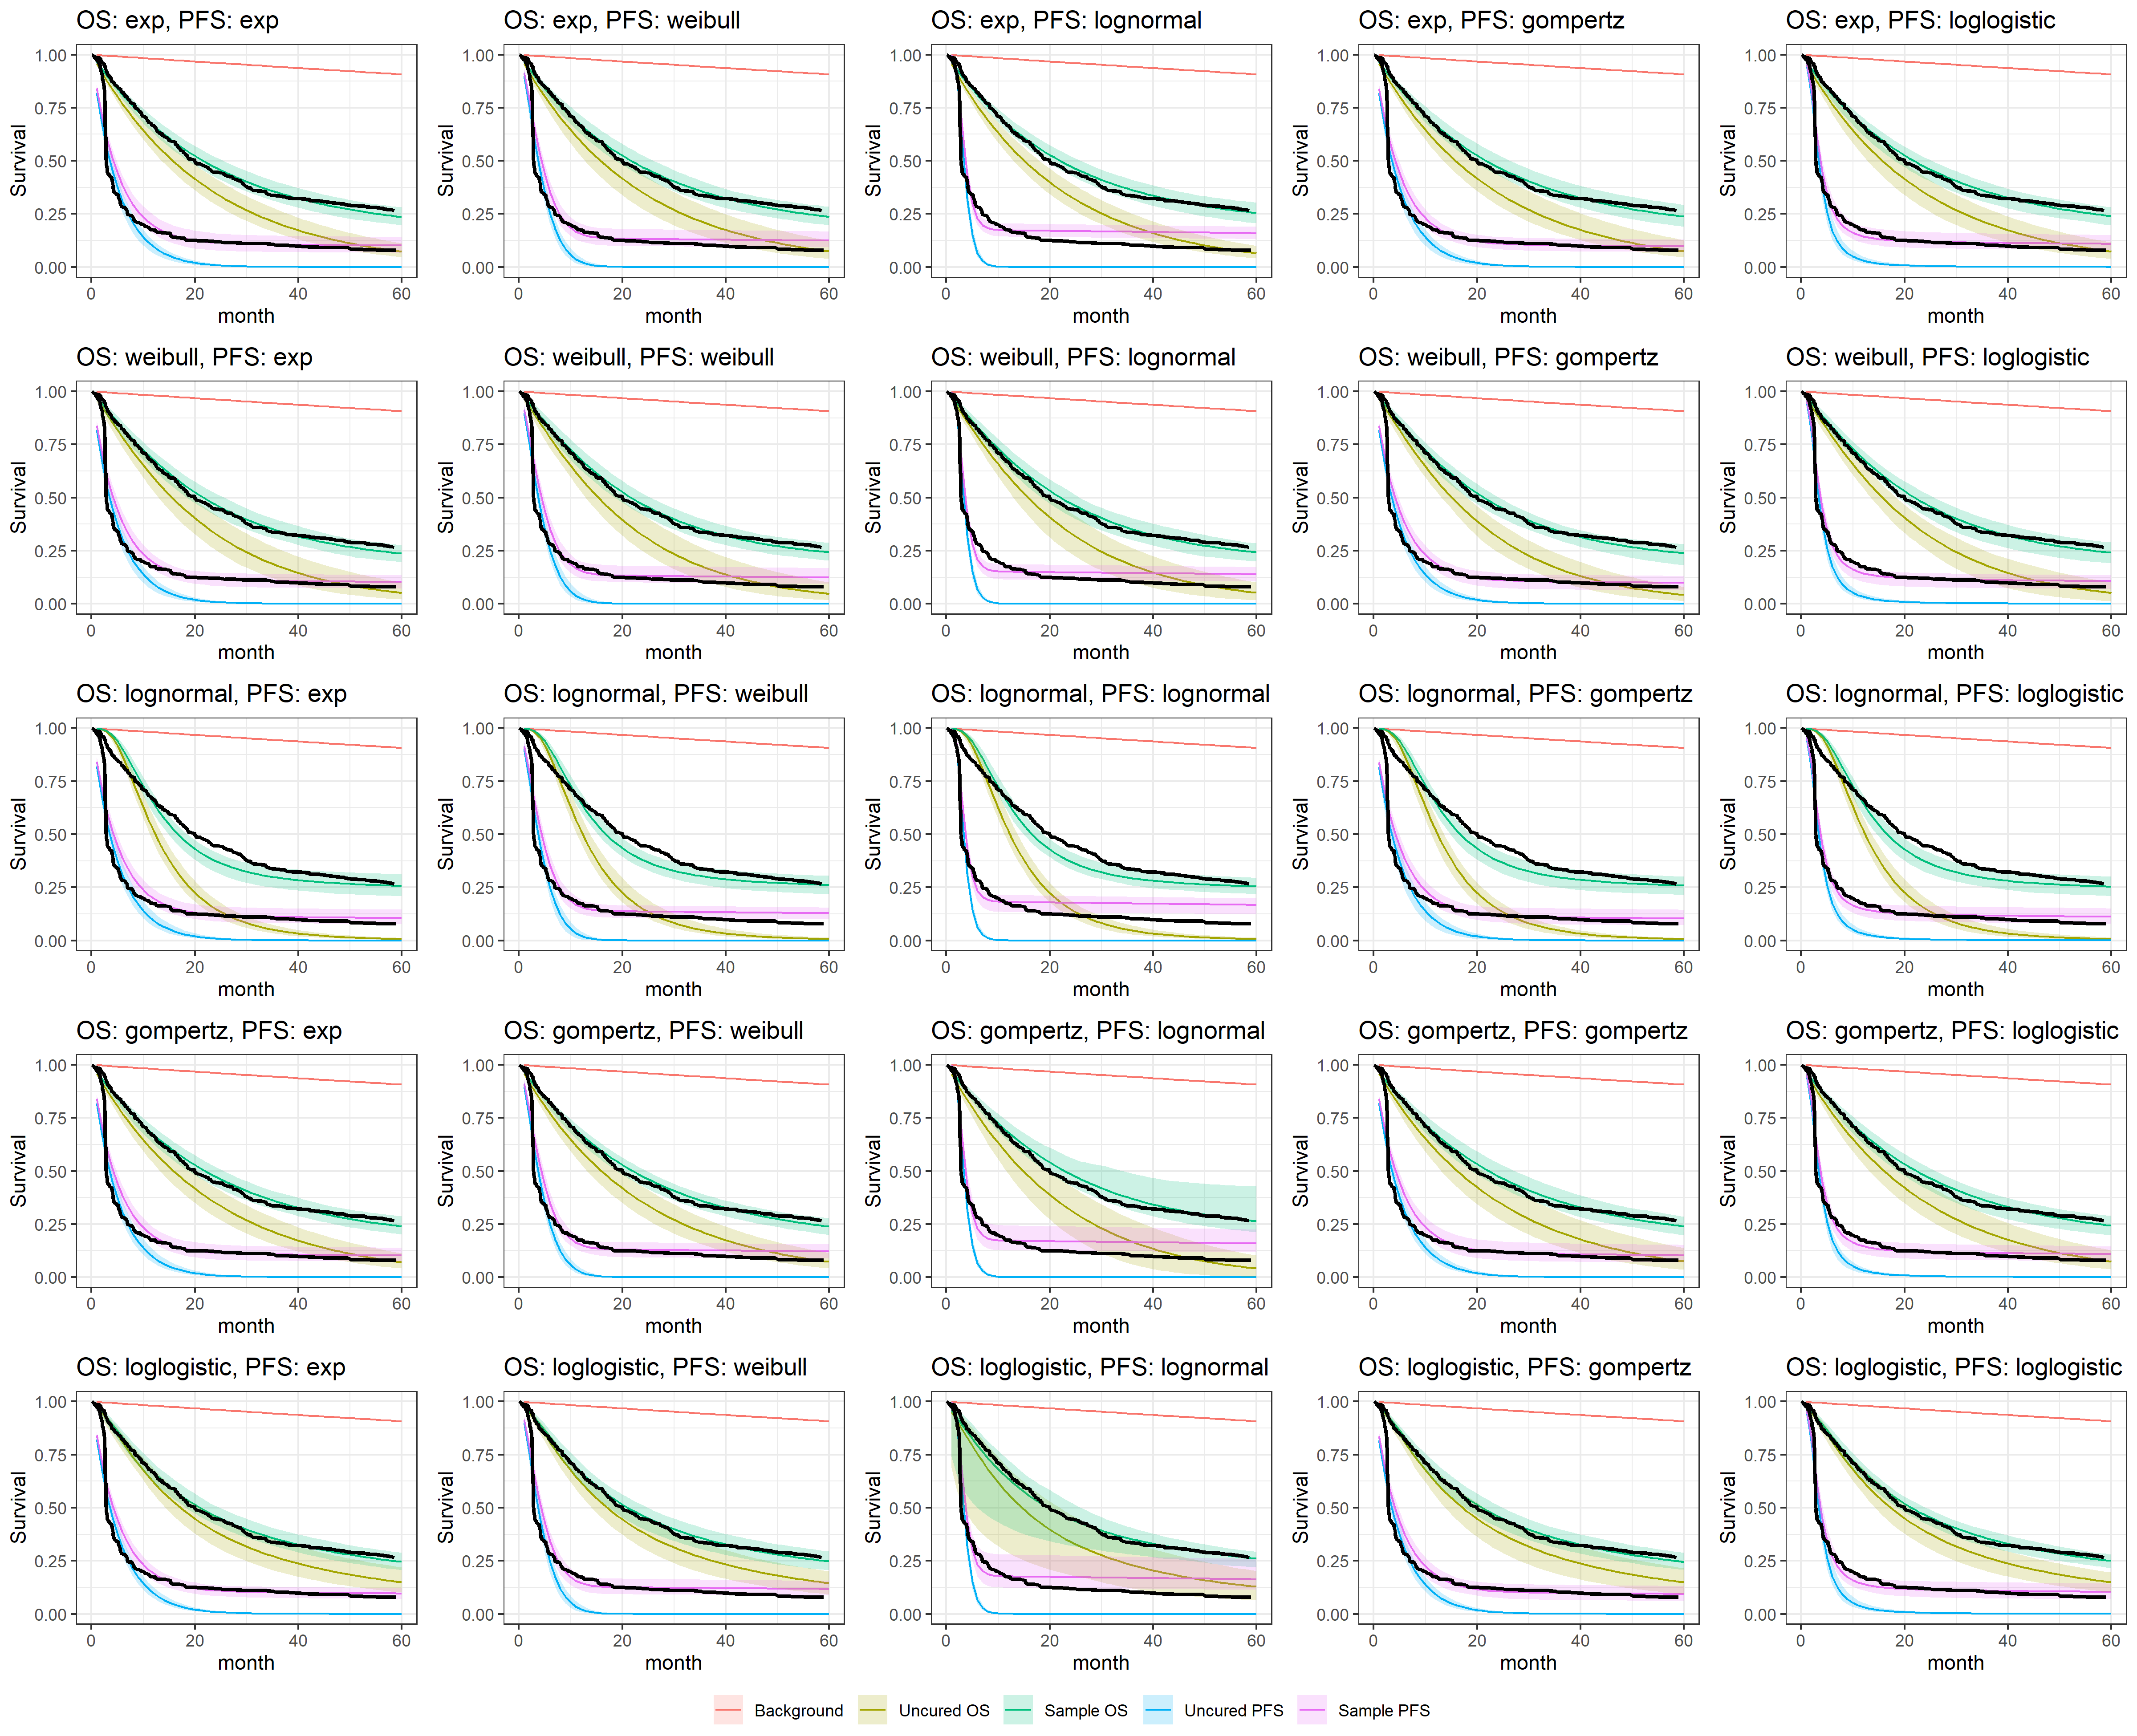
\includegraphics[width=0.9\linewidth]{plot_S_grid_IPILIMUMAB.png}
\caption{\label{fig:S_grid_ipi} Posterior survival curves for exponential, weibull, gompertz, log-logistic and log-Normal uncured fraction for OS and PFS events and {\it ipilimumab} treatment.}
\end{sidewaysfigure}

\begin{sidewaysfigure}[H]
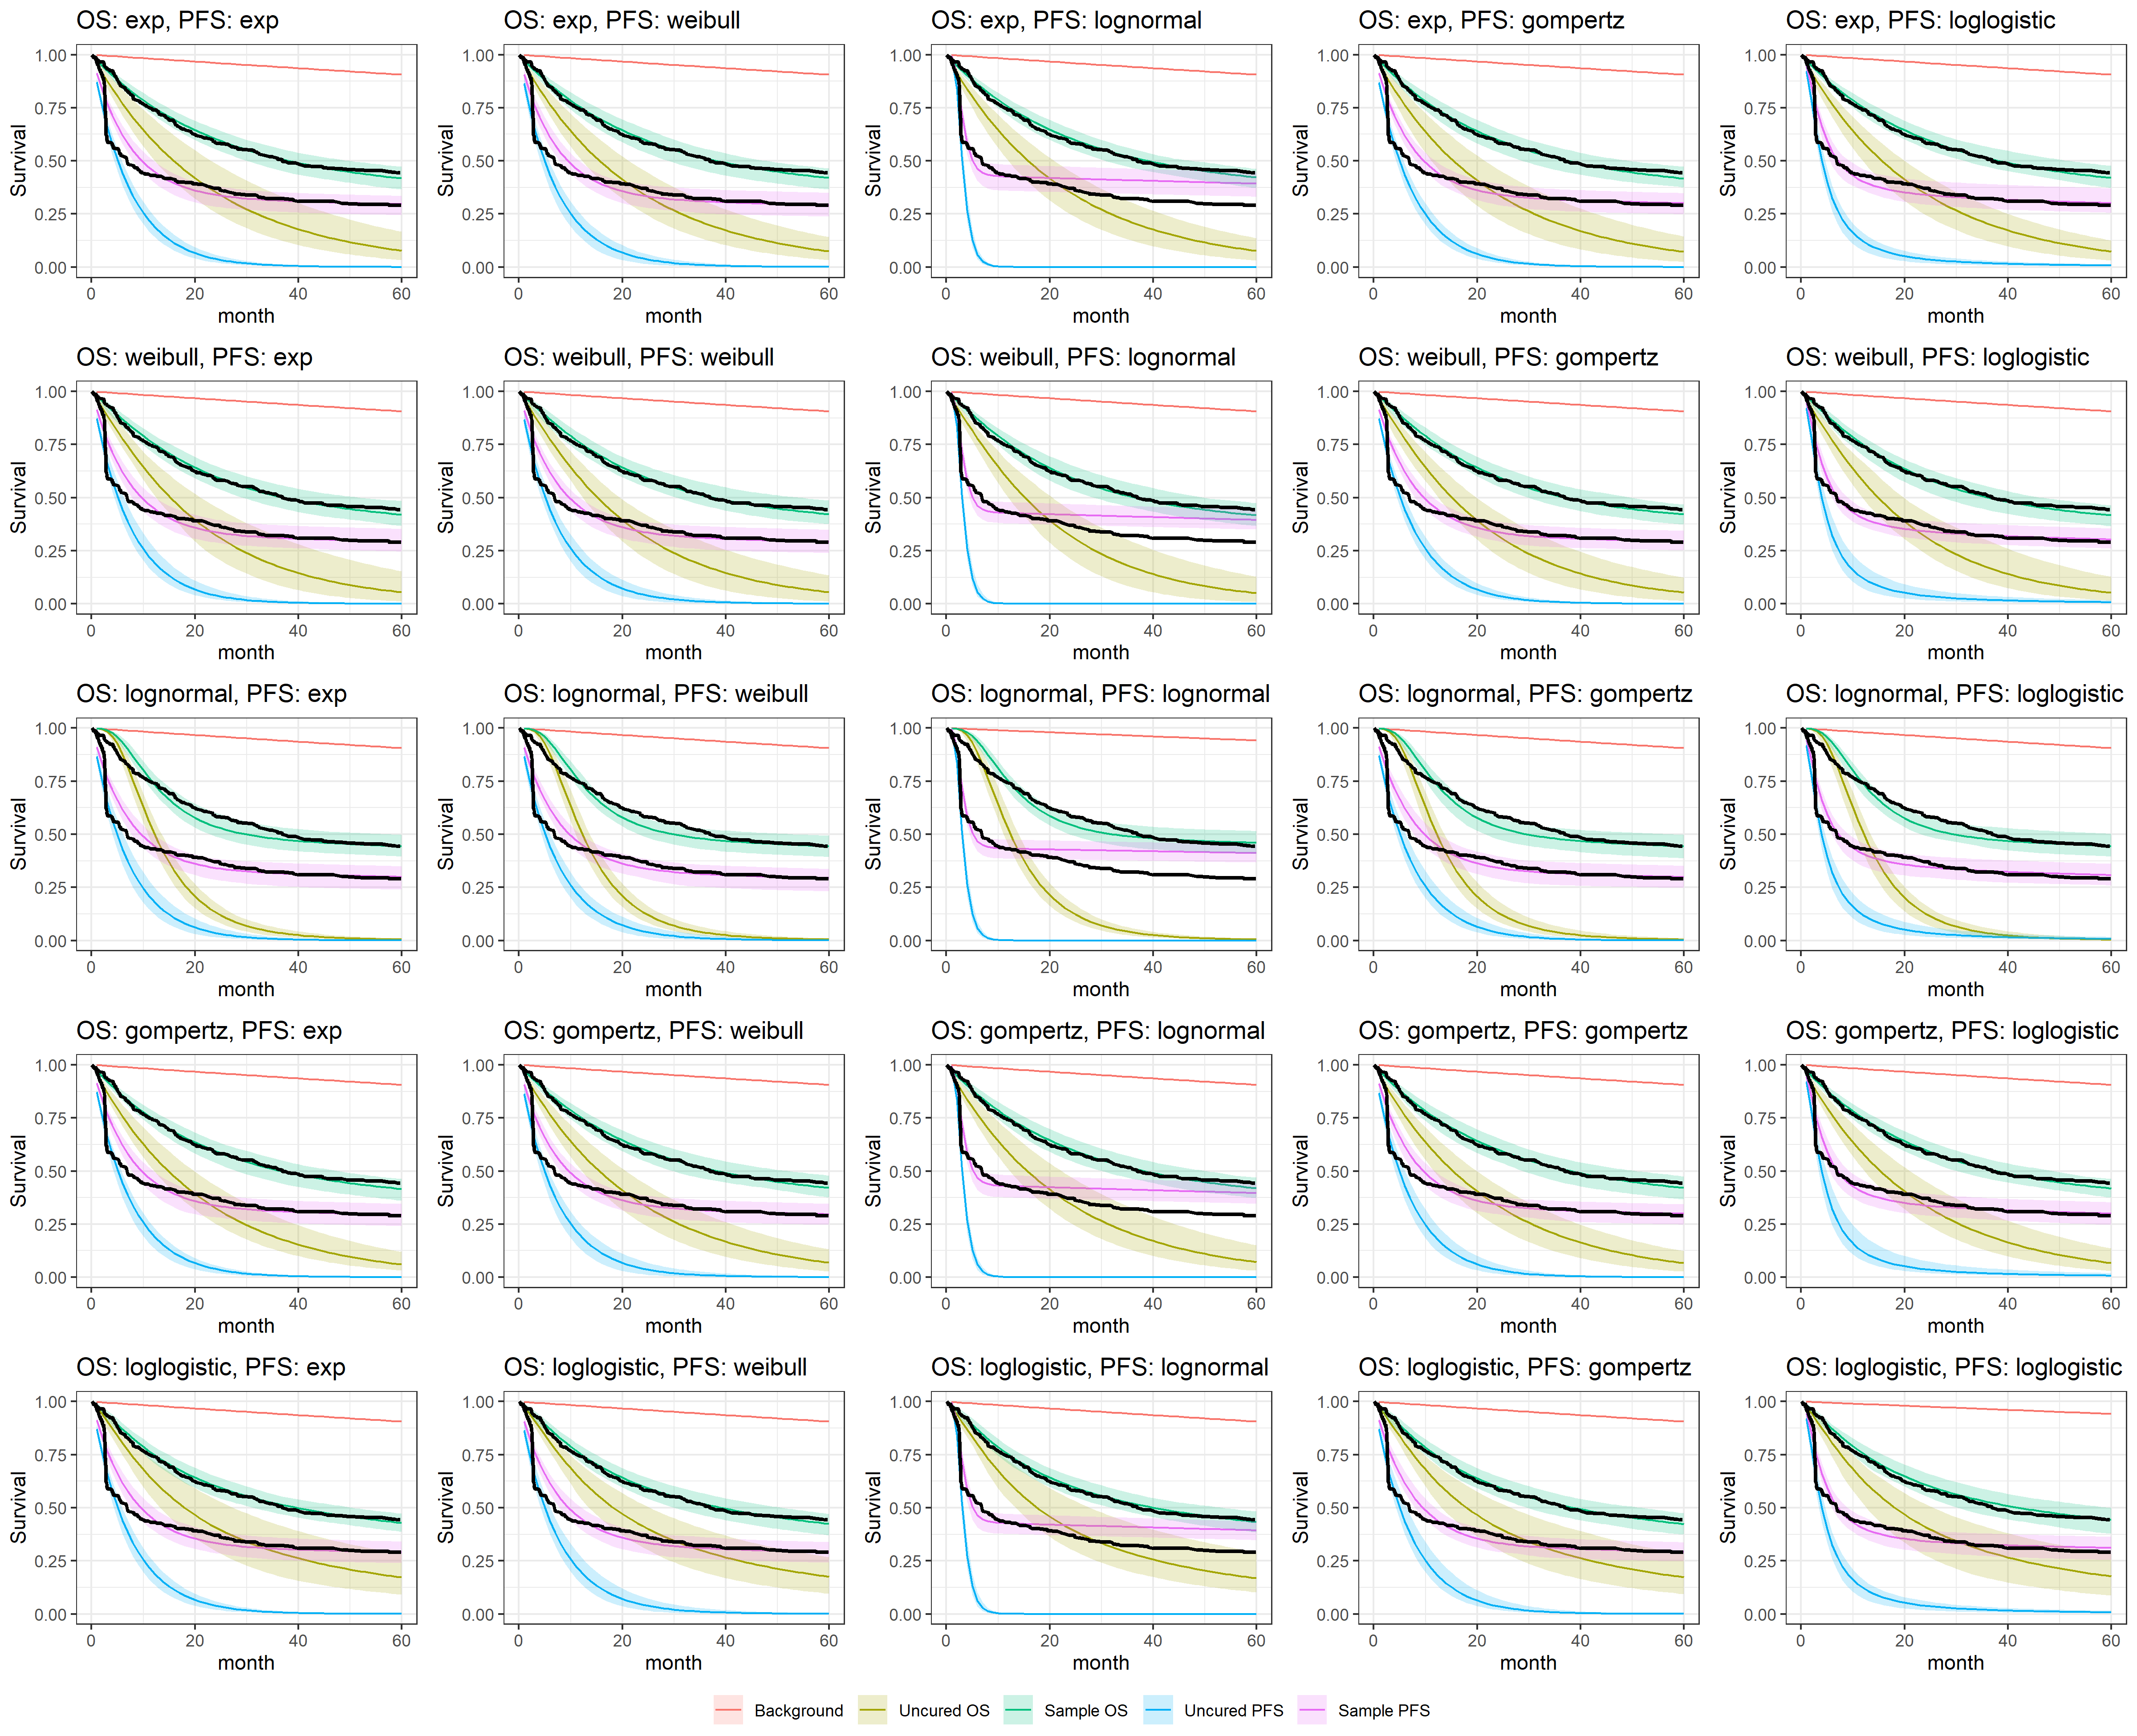
\includegraphics[width=0.9\linewidth]{plot_S_grid_NIVOLUMAB.png}
\caption{\label{fig:S_grid_nivo} Posterior survival curves for exponential, weibull, gompertz, log-logistic and log-Normal uncured fraction for OS and PFS events and {\it nivolumab} treatment.}
\end{sidewaysfigure}

% \begin{figure}[H]
% \centering
% 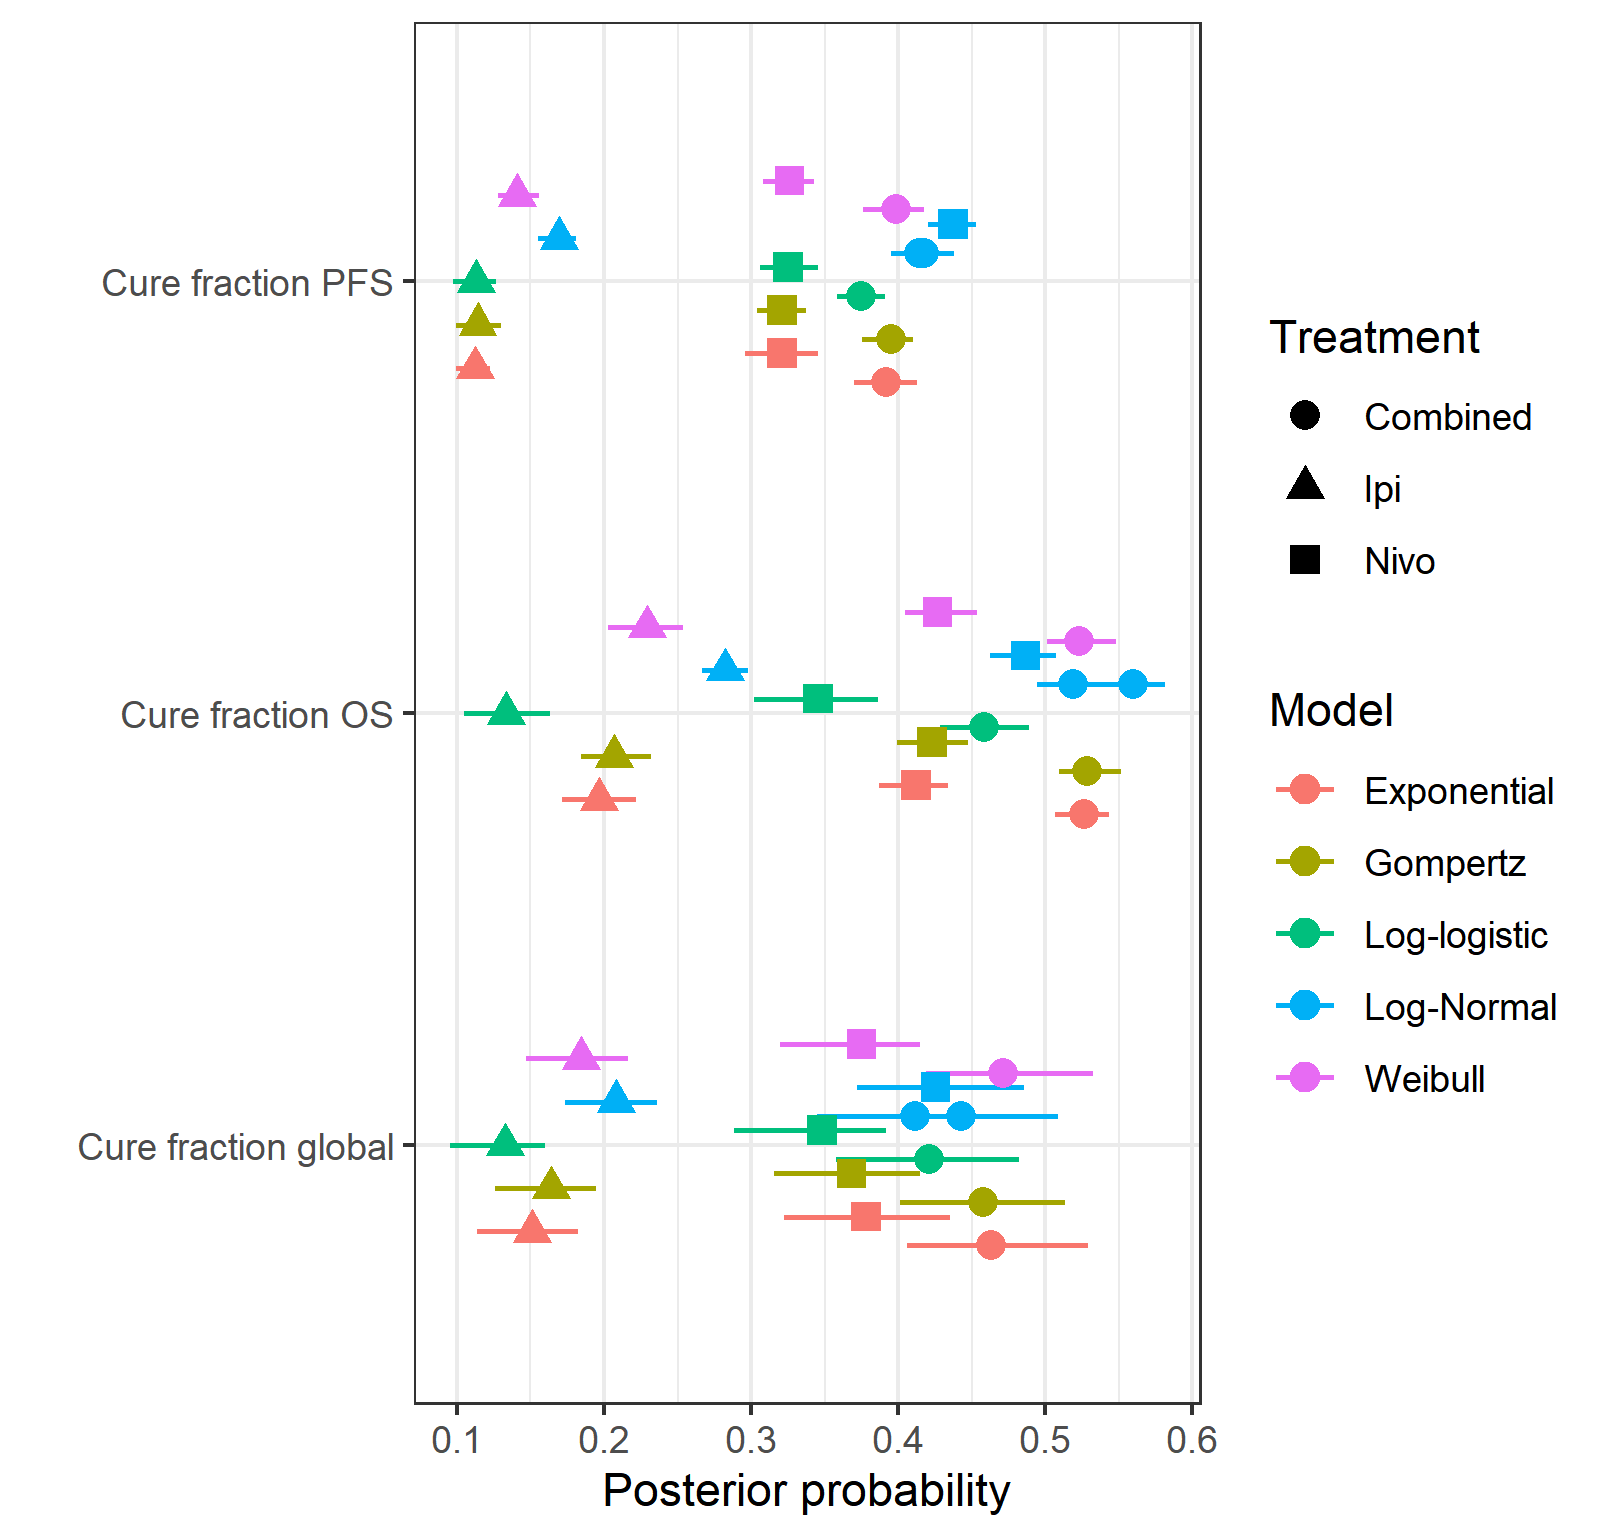
\includegraphics[width=0.6\linewidth]{cf hier_bg_fixed_forest_plot.png}
% \caption{\label{fig:cf_forest} Posterior cure fraction forest plot. Same distributions for OS and PFS. {\it is this how we want to split this up? E.g. do we want different OS and PFS distributions and same treatment? Or separate plots for each cure fraction type?}}
% \end{figure}

\begin{figure}[H]
\centering
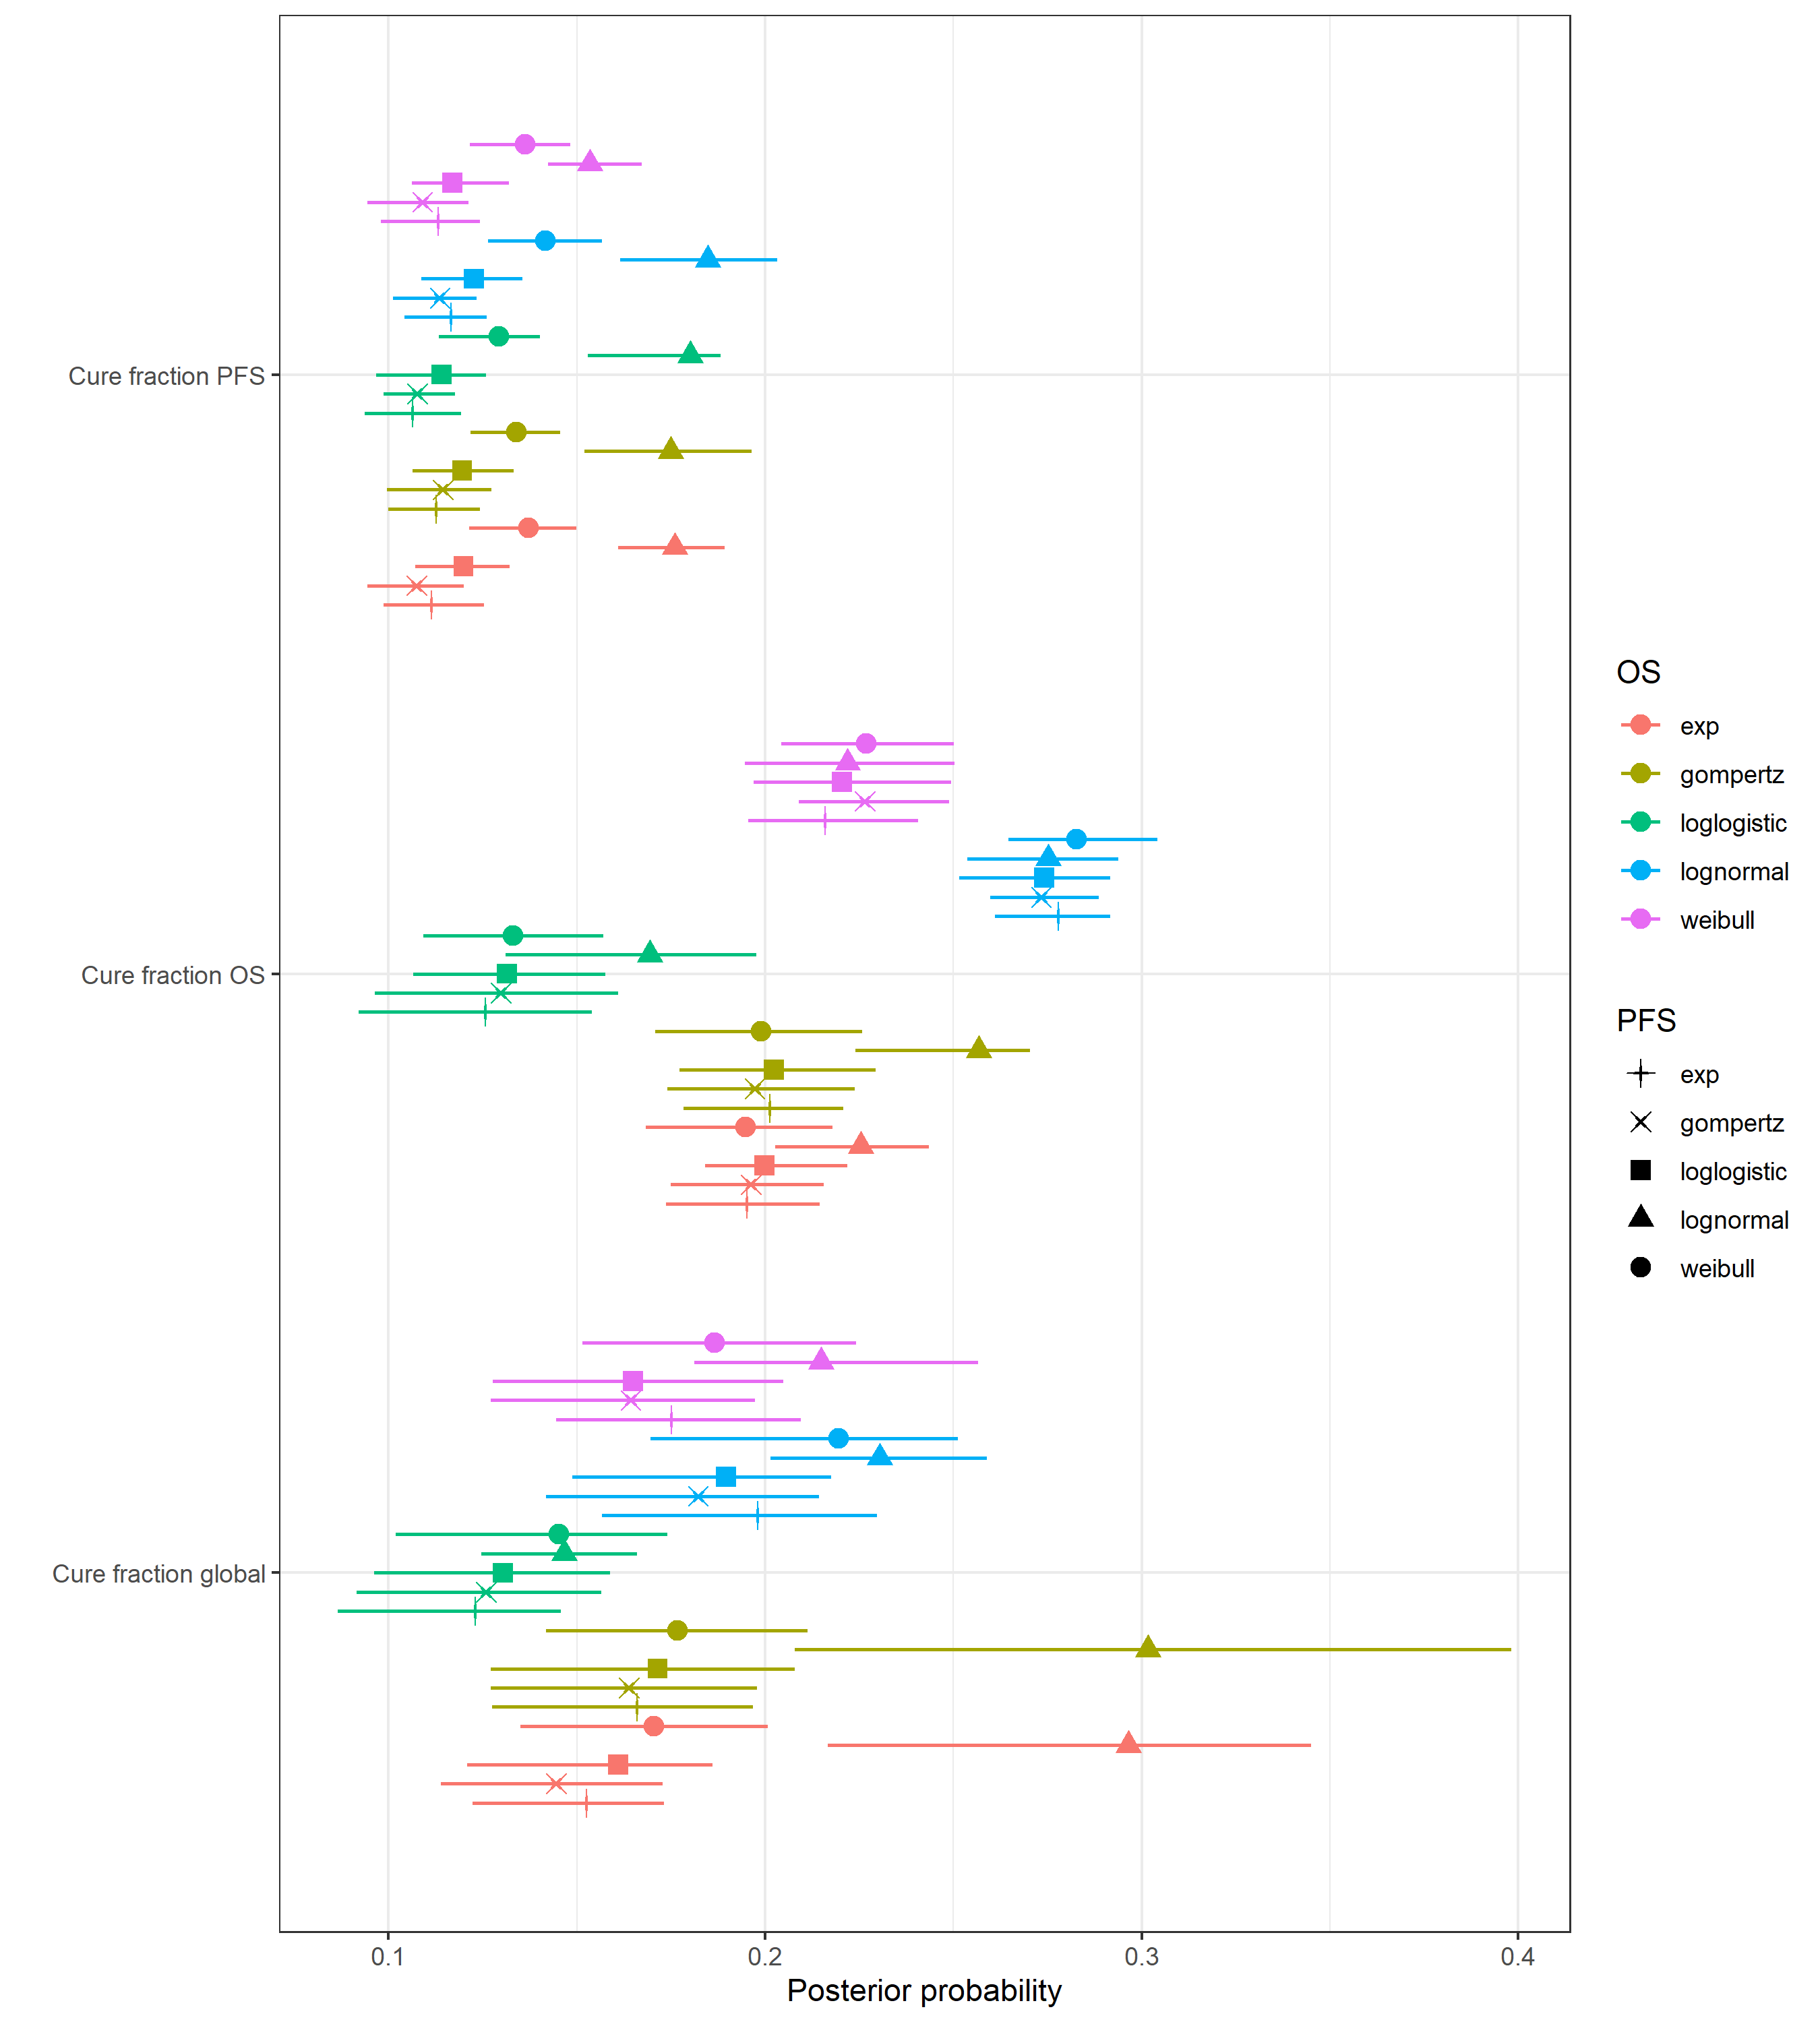
\includegraphics[width=0.6\linewidth]{forest_plot_IPILIMUMAB.png}
\caption{\label{fig:cf_forest_ipi} Posterior cure fraction forest plot for {\it ipilimumab} treatment.}
\end{figure}

\begin{figure}[H]
\centering
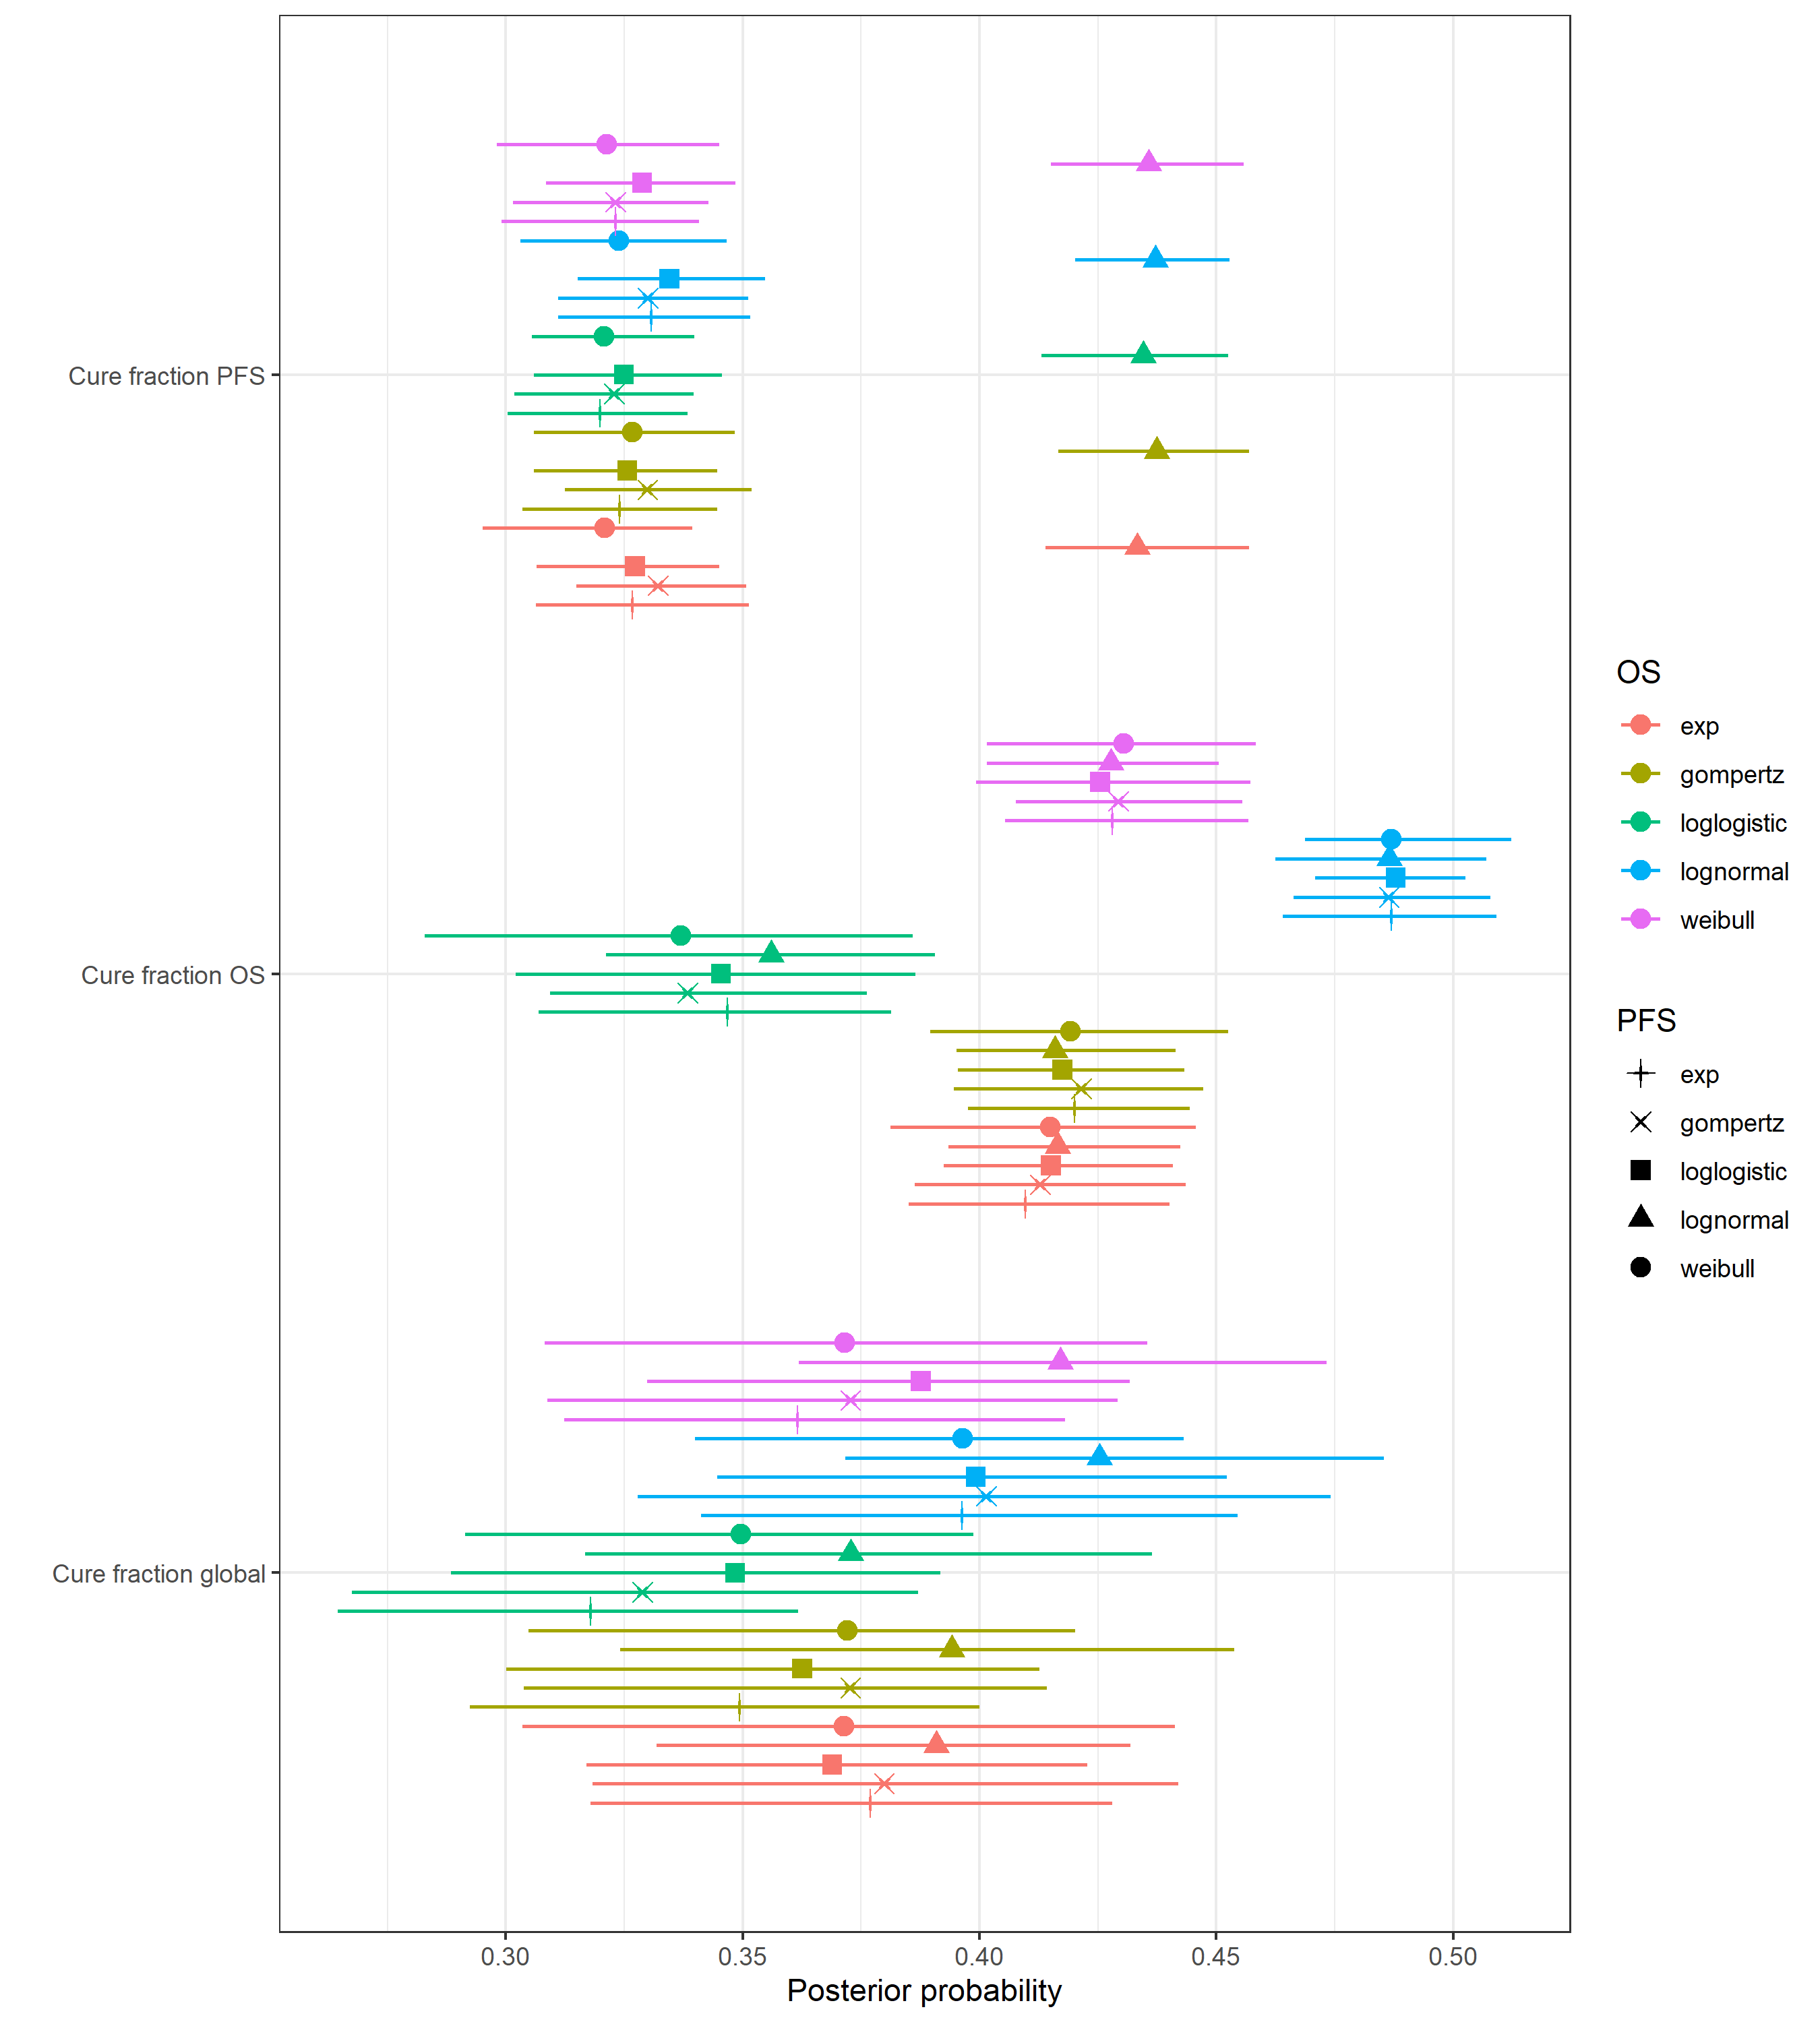
\includegraphics[width=0.6\linewidth]{forest_plot_NIVOLUMAB.png}
\caption{\label{fig:cf_forest_nivo} Posterior cure fraction forest plot for {\it nivolumab} treatment.}
\end{figure}

\begin{figure}[H]
\centering
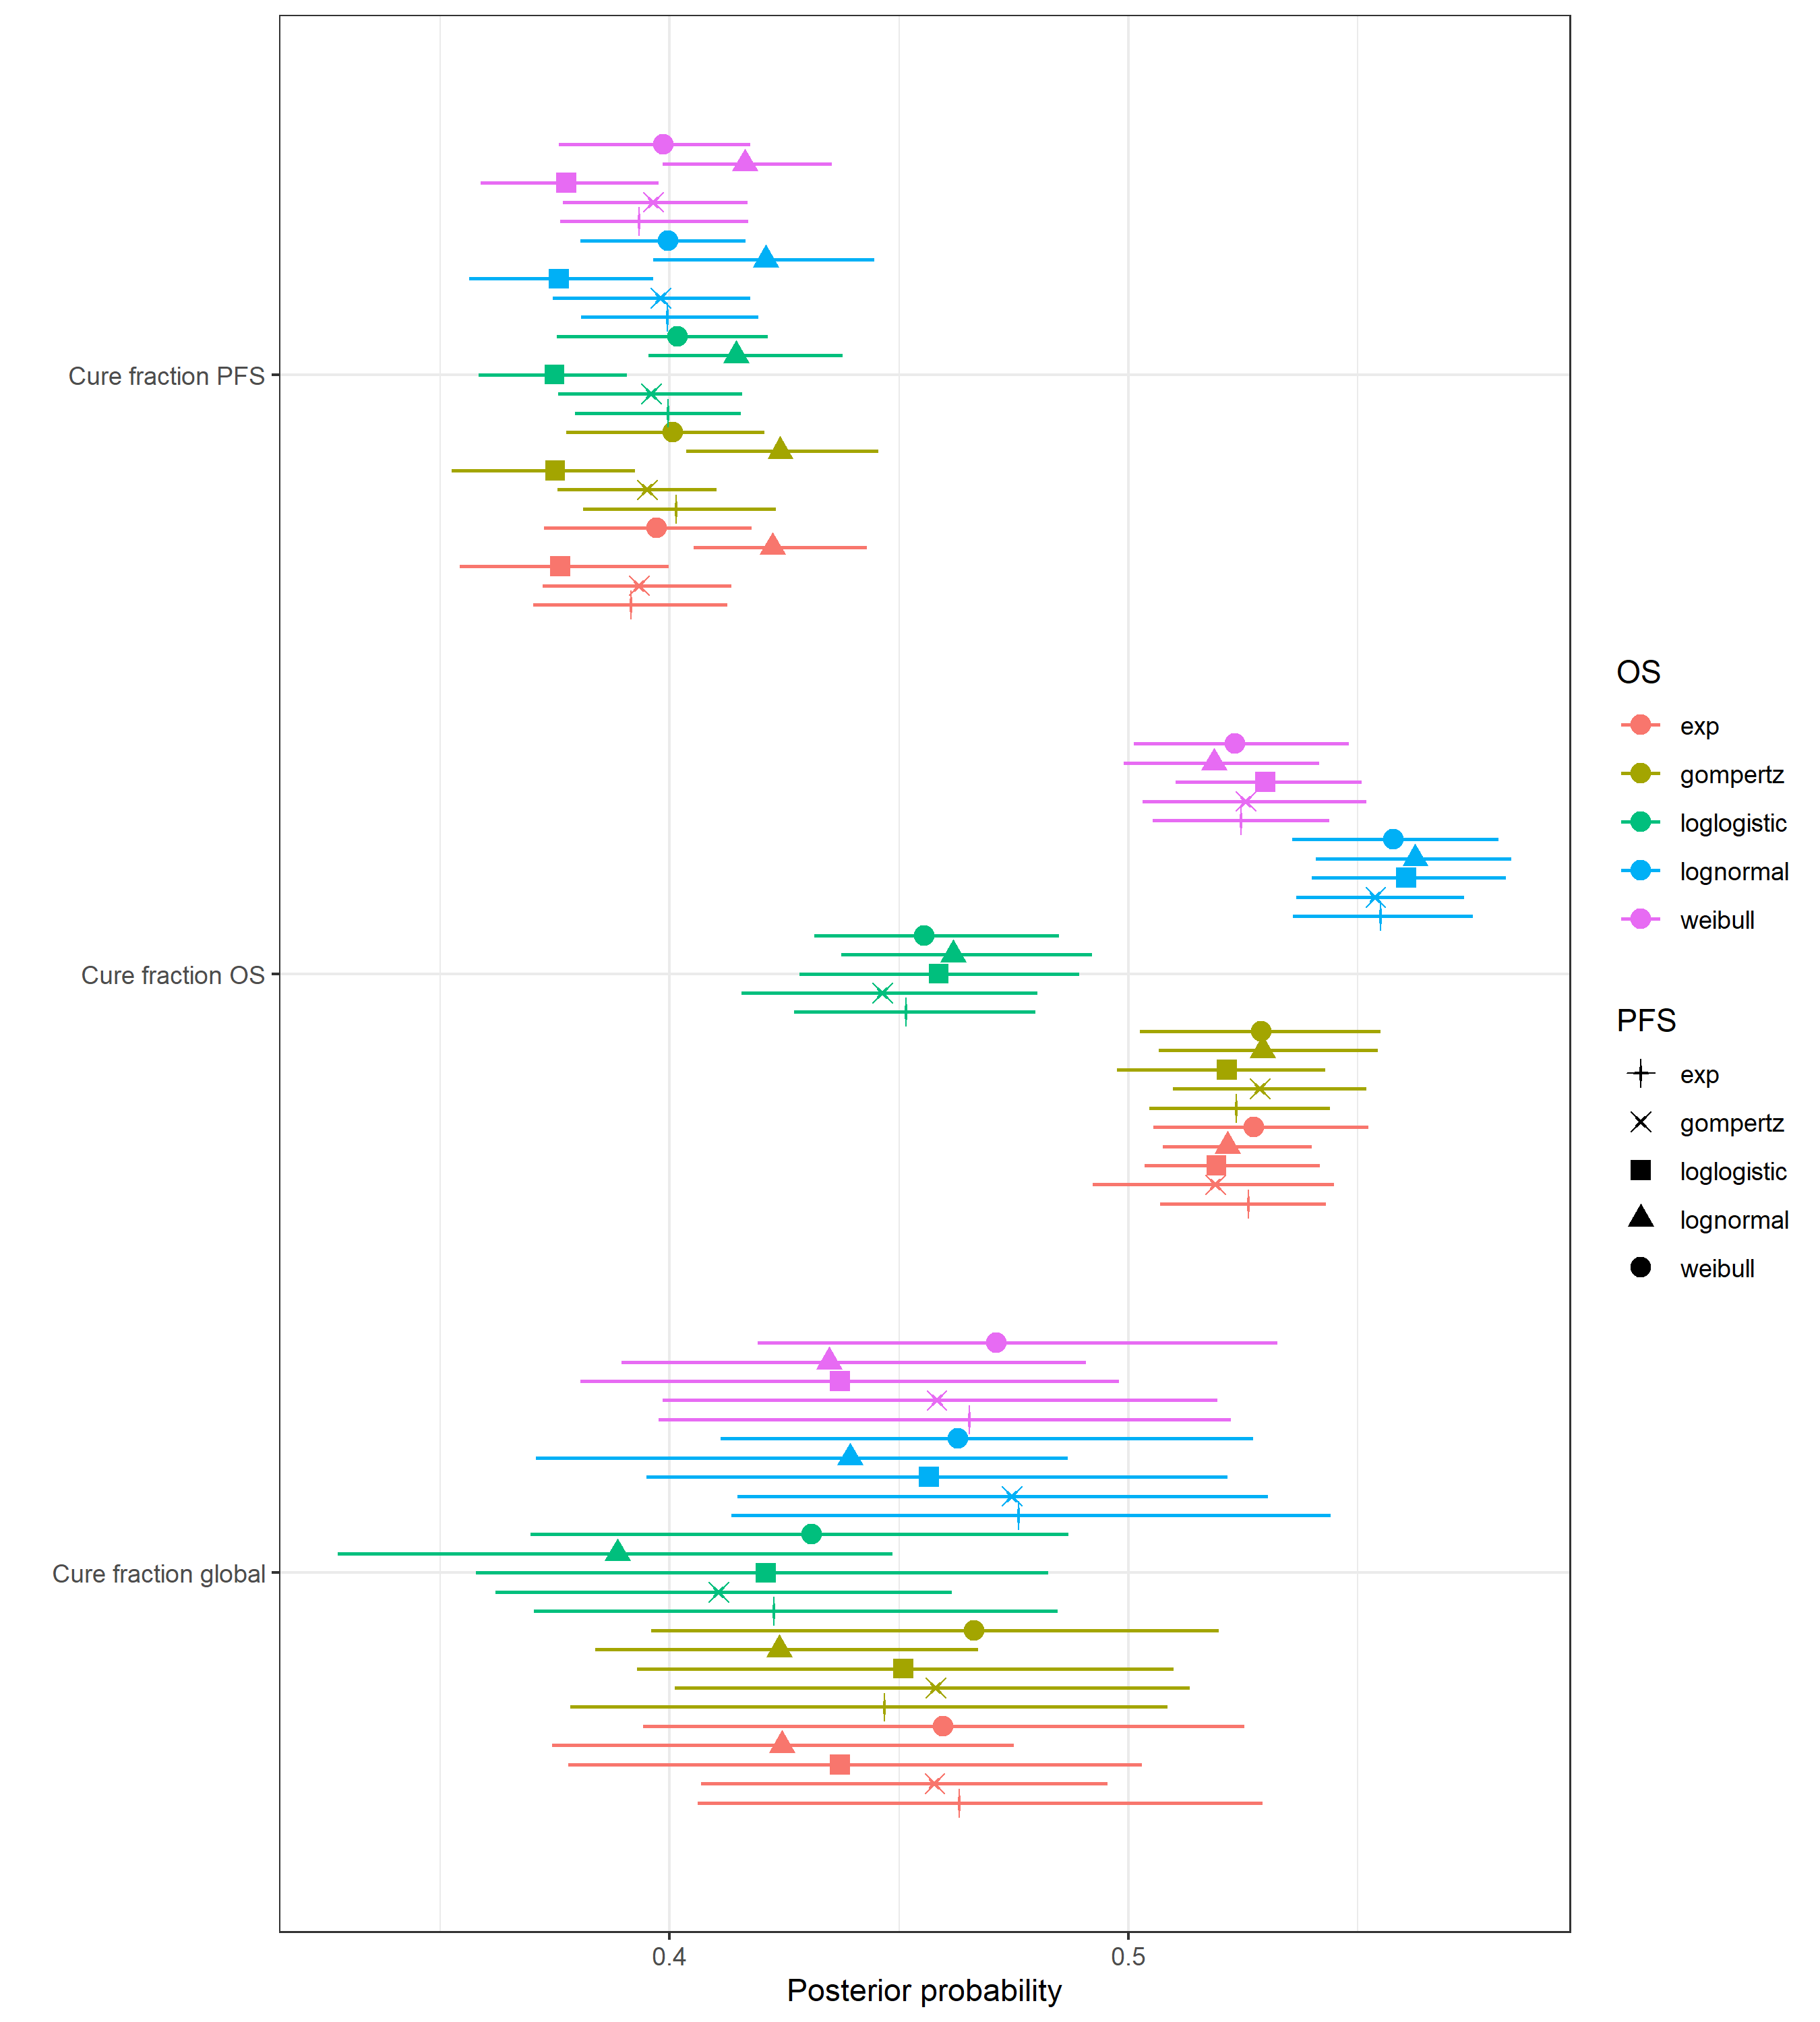
\includegraphics[width=0.6\linewidth]{forest_plot_NIVOLUMAB+IPILIMUMAB.png}
\caption{\label{fig:cf_forest_ipi_nivo} Posterior cure fraction forest plot for {\it nivolumab} and {\it ipilimumab} combination treatment.}
\end{figure}


\subsection{PFS and OS modelled separately}
\subsection{Exchangeable cure fraction}
\subsubsection{Treatments modelled separately}
\subsubsection{Treatments modelled jointly}

Exponential, Weibull, Gompertz, Log-Normal, Log-Logistic\\
{\it model assessment?}



\section{Discussion}\label{sec:discussion}

Our approach allows for the incorporation of sensible information.
Stabilise the inference on the cure fraction but restricting/constraining it values via the prior distributions.
The priors can be specified on the natural scale to aid elicitation and interpretation.


%\backmatter

\section*{Acknowledgements}
This is acknowledgement text.

\subsection*{Author contributions}

This is an author contribution text.

\subsection*{Financial disclosure}

None reported.

\subsection*{Conflict of interest}

The authors declare no potential conflict of interests.


% \section*{Supporting information}

% The following supporting information is available as part of the online article:

% \noindent
% \textbf{Figure S1.}
% {500{\uns}hPa geopotential anomalies for GC2C calculated against the ERA Interim reanalysis. The period is 1989--2008.}


% \appendix

% \section{Section title of first appendix\label{app1}}

% with normal text font. Refer below example:

% \begin{lstlisting}[caption={Descriptive Caption Text},label=DescriptiveLabel]
% for i:=maxint to 0 do
% \end{lstlisting}

% %\nocite{*}% Show all bib entries - both cited and uncited; comment this line to view only cited bib entries;
\bibliography{bibliography}

% \clearpage

% \section*{Author Biography}

% \begin{biography}{
\includegraphics[width=66pt,height=86pt,draft]{empty}}{\textbf{Author Name.} This is sample author is sample author biography text.}
% \end{biography}

\end{document}
